% Slides accompanying "Learn RISC-V CPU Implementation and BSV" book
% Copyright (c) 2024 Rishiyur S. Nikhil, All Rights Reserved

% -*- mode: fundamental -*-

% Slides accompanying "Learn RISC-V CPU Implementation and BSV" book
% Copyright (c) 2024 Rishiyur S. Nikhil, All Rights Reserved

% This is a preamble shared by all the slide decks

\documentclass[10pt, aspectratio=169]{beamer}

% \documentclass[17pt]{beamer}

% Avail. font sizes: 8pt, 9pt, 10pt, 11pt, 12pt, 14pt, 17pt, 20pt.
% Default font size is 11pt (= 22pt in full screen mode).

\usepackage{verbatim}
\usepackage{fancyvrb}
\usepackage{listings}

% ================================================================
% Themes

\usetheme{Madrid}          % Line at bottom: Author (affiliation), OptTitle, Conf, page 

% \usetheme{Copenhagen}    % Same as Madrid except bottom line: Author, OptTitle

% \usetheme{Berkeley}    % Takes up 1-inch border on left and top

% ----------------
% colorthemes
% (default), beaver, beetle, seahorse, wolverine

\usecolortheme{seahorse}

% ================================================================
% Customization: show table of contents before each section
% Use \AtBeginSubsection    to show before each subsection

% \AtBeginSection[]
% {
%   \begin{frame}
%     \frametitle{Table of Contents}
%     \tableofcontents[currentsection]
%   \end{frame}
% }

% ================================================================

% ----------------
% The bsc compiler and BSV language
\newcommand{\bsc}{\emph{bsc}}
\newcommand{\BSV}{\bf{BSV}}
% ----------------
% ITALICISE WORDS
\newcommand{\ie}{\emph{i.e.,}}
\newcommand{\eg}{\emph{e.g.,}}
\newcommand{\Eg}{\emph{E.g.,}}
\newcommand{\etc}{\emph{etc.}}
\newcommand{\via}{\emph{via}}
\newcommand{\vs}{\emph{vs.}}

% ----------------
% EMPTY BOXES OF VARIOUS WIDTHS, FOR INDENTATION

\newcommand{\hm}{\hspace*{1em}}
\newcommand{\hmm}{\hspace*{2em}}
\newcommand{\hmmm}{\hspace*{3em}}
\newcommand{\hmmmm}{\hspace*{4em}}

% ----------------
% Convenient widths

\newlength{\hlessmm}
\setlength{\hlessmm}{\textwidth}
\addtolength{\hlessmm}{-2em}

\newlength{\hlessmmm}
\setlength{\hlessmmm}{\textwidth}
\addtolength{\hlessmmm}{-3em}

\newlength{\hlessmmmm}
\setlength{\hlessmmmm}{\textwidth}
\addtolength{\hlessmmmm}{-4em}

% ================================================================
% Title page

\title[Learn CPU design \& BSV]{Learn RISC-V CPU Implementation and BSV}

\subtitle{(BSV: a High-Level Hardware Design Language)}

\author[{\copyright} R.S.Nikhil]{Rishiyur S.~Nikhil}
% \institute{Bluespec, Inc.}

% Date is set differently in each slide deck

% \logo{
\includegraphics[height=0.6cm]{../Figures/Bluespec_Logo_2022-10}}

% End of preamble
% ****************************************************************


\date{L16: RISC-V: The Fife pipelined CPU}

% ****************************************************************

\begin{document}

% ================================================================

\begin{frame}
\titlepage

\begin{center}
 
\includegraphics[height=1cm]{Bluespec_Logo_2022-10}
\end{center}

\end{frame}

% ================================================================

\section{Reminders}

% -*- mode: fundamental -*-

% ================================================================

\begin{frame}[fragile]
\frametitle{Reminders}

\footnotesize

Please git clone: \url{https://github.com/rsnikhil/Learn_Bluespec_and_RISCV_Design} \\
(git pull for latest version).  Repsitory structure:

\vspace{1ex}

\begin{minipage}{0.5\textwidth}\scriptsize
\begin{Verbatim}[frame=single, numbers=left]
    ./Book_BLang_RISCV.pdf
      Slides/
          Slides_01_Intro.pdf
          Slides_02_ISA.pdf
          ...
      Exercises/
          Ex-03-A-Hello-World/
          Ex-03-B-Top-and-DUT/
          ...
      Code/
          src_Top/
          src_Drum/
          src_Fife/
          src_Common/
          ...
      Doc/Installing_bsc_Verilator_etc.{adoc,html}
\end{Verbatim}
\end{minipage}
\hm
\begin{minipage}{0.45\textwidth}
\begin{itemize}

 \item Slides and Exercise are numbered in sync with book Chapter numbers.

 \item For Exercises, please see Appendix E of the book.  Some (not
       all) exercises have associated code in the {\tt Exercises/}
       directory.

\end{itemize}
\end{minipage}

\vspace{2ex}

To compile and run the code for exercises, Drum and Fife, please make sure you have installed:

\begin{itemize}

 \item \emph{bsc} compiler (see \url{https://github.com/B-Lang-org/bsc})

 \item Verilator compiler (see \url{https://www.verilator.org/})
\end{itemize}

\footnotesize

\end{frame}

% ================================================================

\begin{frame}
\frametitle{Chapter Roadmap}

\footnotesize

\begin{center}
\frame{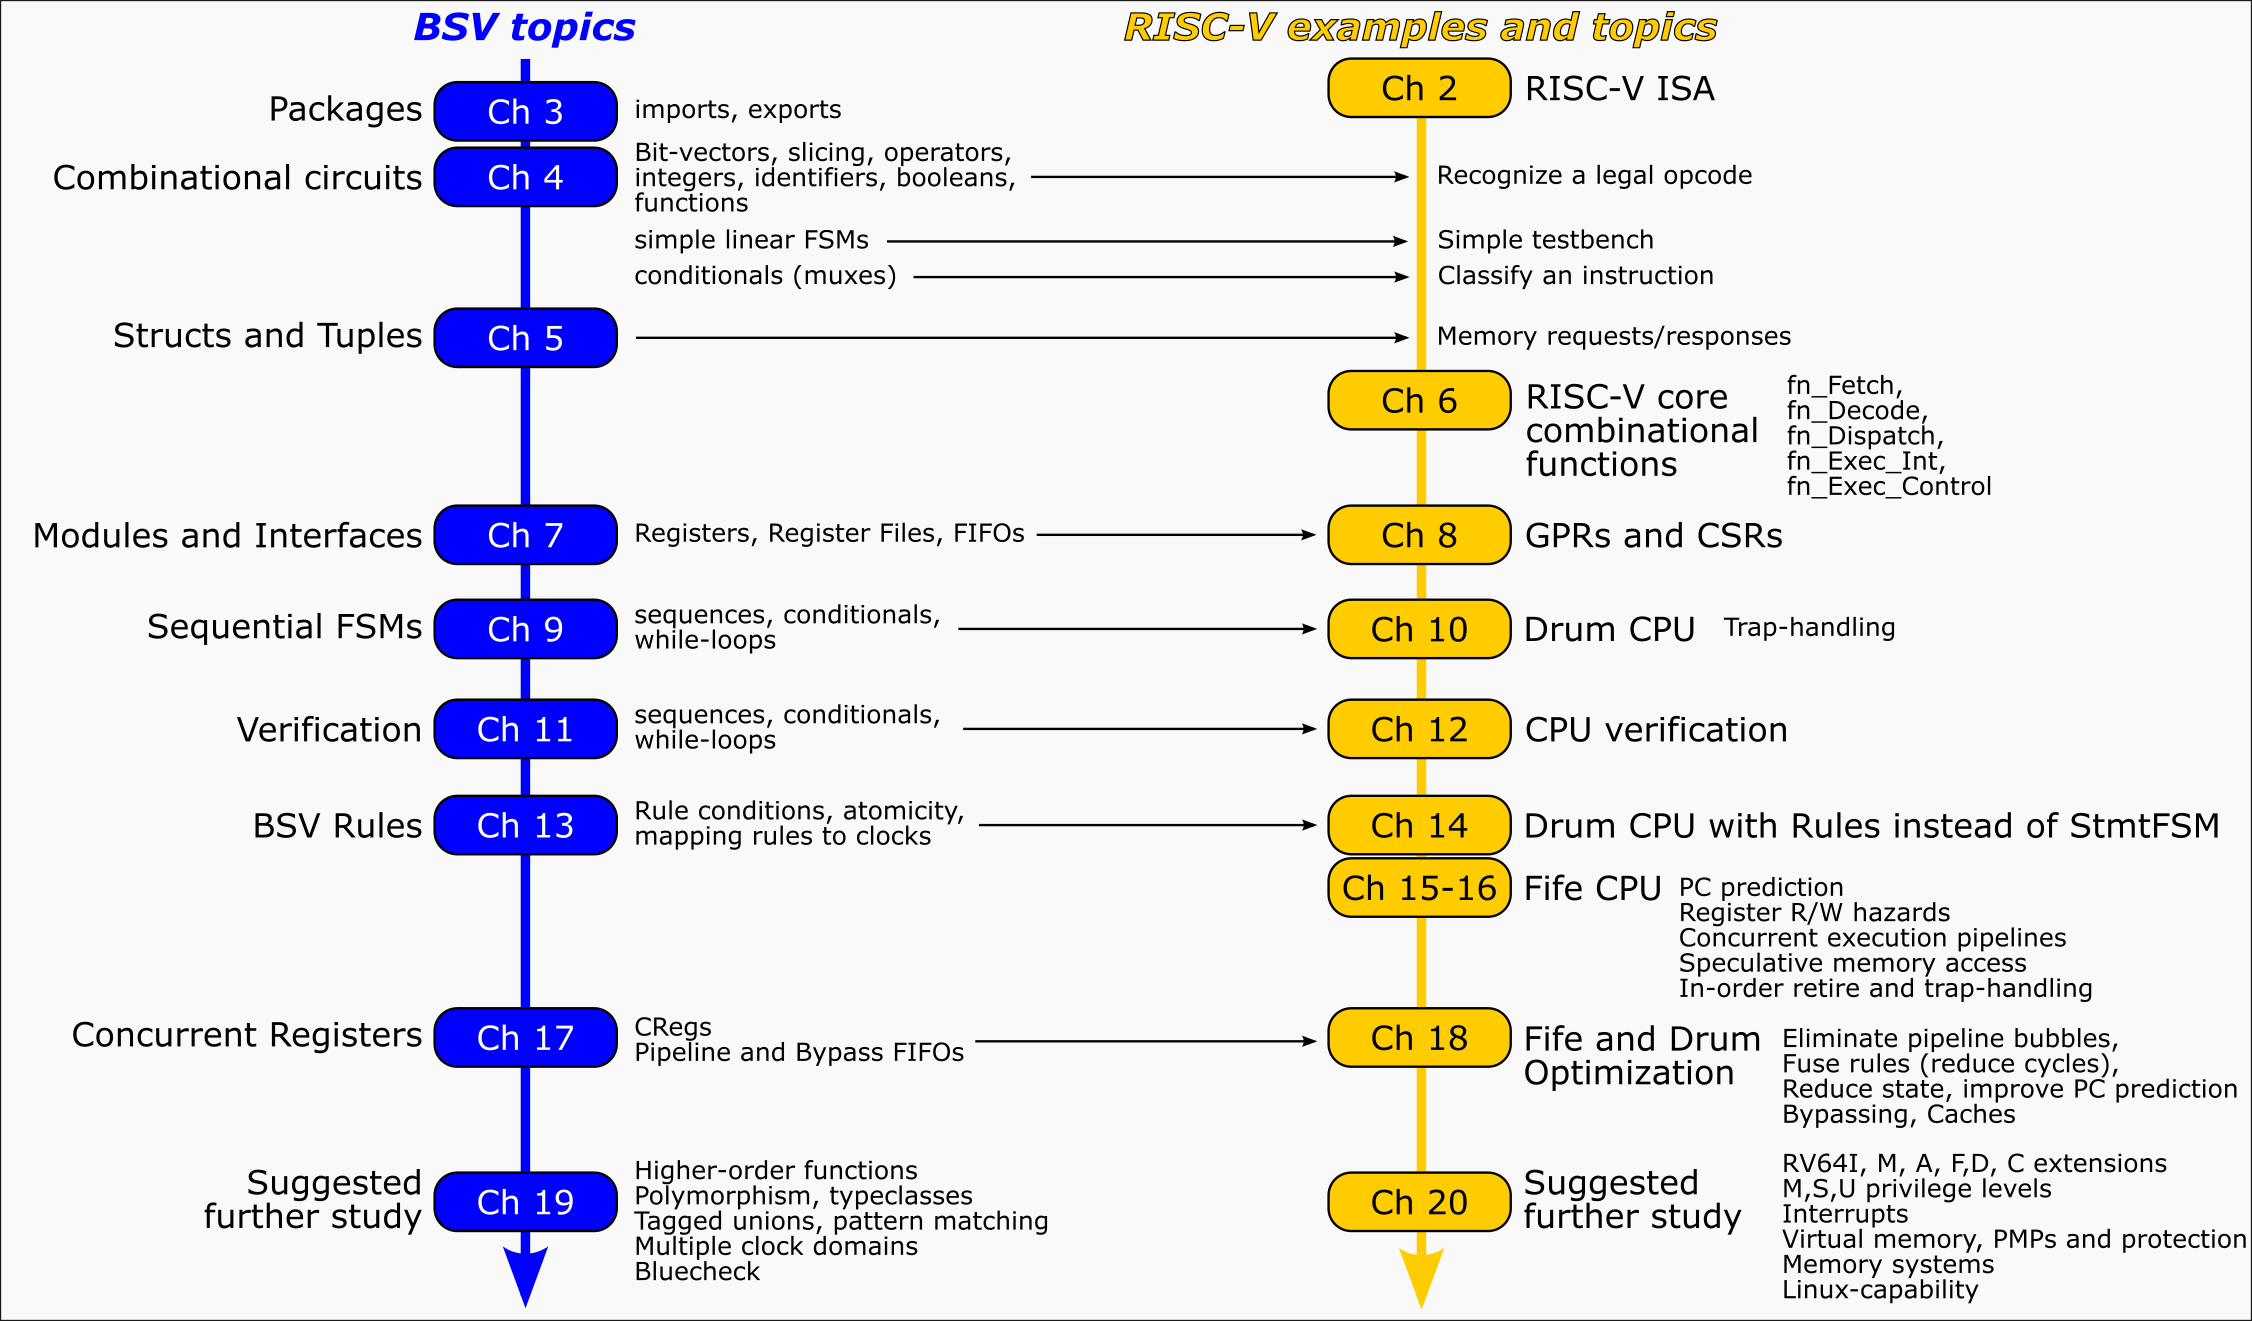
\includegraphics[height=0.825\textheight]{Fig_Chapter_Roadmap}}
\end{center}

\end{frame}

% ================================================================


% ================================================================

\begin{frame}
\frametitle{Flow of information between stages in Drum and Fife}

\label{Slide_Instr_Steps}

\footnotesize

\begin{center}
 \includegraphics[height=0.6\textheight]{Fig_Instr_Exec_w_FIFOs}
\end{center}

\end{frame}

% ================================================================

\begin{frame}
\frametitle{Table of Contents}

\tableofcontents

\end{frame}

% ****************************************************************

\section{Module Interface (same for Drum and Fife)}

\begin{frame}

\begin{center}
  {\LARGE Fife CPU: Module Interface (same for Drum and Fife)}
\end{center}

\end{frame}

% ================================================================

\begin{frame}[fragile]
\frametitle{Module Interface}

\footnotesize


% \SHOWCODE{../Code_Extracts/CPU_IFC.tex}
% TODO: Fix up code-extraction to extract this automatically from source
% from file 'CPU_IFC.bsv' line 27  tag CPU_IFC
{\scriptsize
\begin{Verbatim}[frame=single, numbers=left, label=src\_Common/CPU\_IFC.bsv: line 27 ...]
interface CPU_IFC;
   method Action init (Initial_Params initial_params);

   // IMem
   interface FIFOF_O #(Mem_Req) fo_IMem_req;
   interface FIFOF_I #(Mem_Rsp) fi_IMem_rsp;

   // DMem, speculative
   interface FIFOF_O #(Mem_Req) fo_DMem_S_req;
   interface FIFOF_I #(Mem_Rsp) fi_DMem_S_rsp;
   interface FIFOF_O #(Retire_to_DMem_Commit)  fo_DMem_S_commit;

   // DMem, non-speculative
   interface FIFOF_O #(Mem_Req) fo_DMem_req;
   interface FIFOF_I #(Mem_Rsp) fi_DMem_rsp;

   // Set TIME
   (* always_ready, always_enabled *)
   method Action set_TIME (Bit #(64) t);
endinterface
\end{Verbatim}
}

\vspace{1ex}

The speculative DMem sub-interfaces: \\
\hmm {\tt fo\_DMem\_S\_req} \hmm {\tt fi\_DMem\_S\_rsp} \hmm {\tt fo\_DMem\_S\_commit} \\
were unused in Drum, and are used in Fife.

\end{frame}

% ****************************************************************

\section{Top-level {\tt mkCPU} module}

\begin{frame}[fragile]

\begin{center}
  {\LARGE Fife CPU: Top-level {\tt mkCPU} module}

  \vspace{10ex}

  Please simultaneously view file: \hm \verb|Code/src_Fife/CPU.bsv|
\end{center}

\end{frame}

% ================================================================

\begin{frame}[fragile]
\frametitle{Overall Fife CPU module structure}

\footnotesize

\begin{minipage}{0.725\textwidth}
\begin{Verbatim}[frame=single, label=From src\_Drum/CPU.bsv]
(* synthesize *)
module mkCPU (CPU_IFC);
   // ****************************************************************
   // STATE (sub-modules for pipeline stages)
   ...

   // ****************************************************************
   // STATE (sub-modules for inter-stage connections)

   ...
   // ****************************************************************
   // INTERFACE
   ...
endmodule
\end{Verbatim}
\end{minipage}
\hm
\emph{Details in slides that follow}

\vspace{5ex}

Fife's {\tt mkCPU} module is actually simpler than Drum's {\tt mkCPU}
because the major functionality is now in the separate stage
sub-modules (Drum did not have stage sub-modules).

\end{frame}

% ================================================================

\begin{frame}[fragile]
\frametitle{Fife module state: sub-modules for pipeline stages}

\footnotesize

\begin{minipage}{0.75\textwidth}
\begin{Verbatim}[frame=single, label=From src\_Fife/CPU.bsv]
   // Pipeline stages
   Fetch_IFC       stage_F          <- mkFetch;
   Decode_IFC      stage_D          <- mkDecode;
   RR_RW_IFC       stage_RR_RW      <- mkRR_RW;
   EX_Control_IFC  stage_EX_Control <- mkEX_Control;  // Branch, JAL, JALR
   EX_Int_IFC      stage_EX_Int     <- mkEX_Int;      // Integer ops
   Retire_IFC      stage_Retire     <- mkRetire;
\end{Verbatim}
\end{minipage}
\hm
\begin{minipage}{0.22\textwidth}
Fife instantiates a sub-module for each of the pipeline stages
\end{minipage}



\end{frame}

% ================================================================

\begin{frame}[fragile]
\frametitle{Fife module state: inter-stage forward-flow connections (sub-modules) }

\footnotesize

\begin{minipage}{0.75\textwidth}\scriptsize
\begin{Verbatim}[frame=single, label=From src\_Fife/CPU.bsv]
   // Forward flow connections

   // Fetch->Decode->RR-Dispatch, and direct path RR-Dispatch->Retire
   mkConnection (stage_F.fo_Fetch_to_Decode,  stage_D.fi_Fetch_to_Decode);
   mkConnection (stage_D.fo_Decode_to_RR,     stage_RR_RW.fi_Decode_to_RR);
   mkConnection (stage_RR_RW.fo_RR_to_Retire, stage_Retire.fi_RR_to_Retire);

   // RR-Dispatch->various EX
   mkConnection (stage_RR_RW.fo_RR_to_EX_Control,
		 stage_EX_Control.fi_RR_to_EX_Control);
   mkConnection (stage_RR_RW.fo_RR_to_EX_Int,
		 stage_EX_Int.fi_RR_to_EX_Int);

   // Various EX->Retire
   mkConnection (stage_EX_Control.fo_EX_Control_to_Retire,
		 stage_Retire.fi_EX_Control_to_Retire);
   mkConnection (stage_EX_Int.fo_EX_Int_to_Retire,
		 stage_Retire.fi_EX_Int_to_Retire);
\end{Verbatim}
\end{minipage}
\hm
\begin{minipage}{0.22\textwidth}
Each connection is a FIFO
\end{minipage}

\end{frame}

% ================================================================

\begin{frame}[fragile]
\frametitle{Fife module state: inter-stage backward-flow connections (sub-modules)}

\footnotesize

\begin{minipage}{0.75\textwidth}\scriptsize
\begin{Verbatim}[frame=single, label=From src\_Fife/CPU.bsv]
   // Backward flow connections

   // Fetch<-Retire (redirection)
   mkConnection (stage_Retire.fo_Fetch_from_Retire, stage_F.fi_Fetch_from_Retire);
   // RR-Dispatch<-Retire (register writeback)
   mkConnection (stage_Retire.fo_RW_from_Retire, stage_RR_RW.fi_RW_from_Retire);
\end{Verbatim}
\end{minipage}
\hm
\begin{minipage}{0.22\textwidth}
Each connection is a FIFO
\end{minipage}

\end{frame}

% ================================================================

\begin{frame}[fragile]
\frametitle{FIFO connections between separately compiled Fife sub-modules}

\footnotesize

\begin{minipage}{0.22\textwidth}
Each inter-stage FIFO {\tt mkConnection} has this form:
\end{minipage}
\hfill
\begin{minipage}{0.75\textwidth}
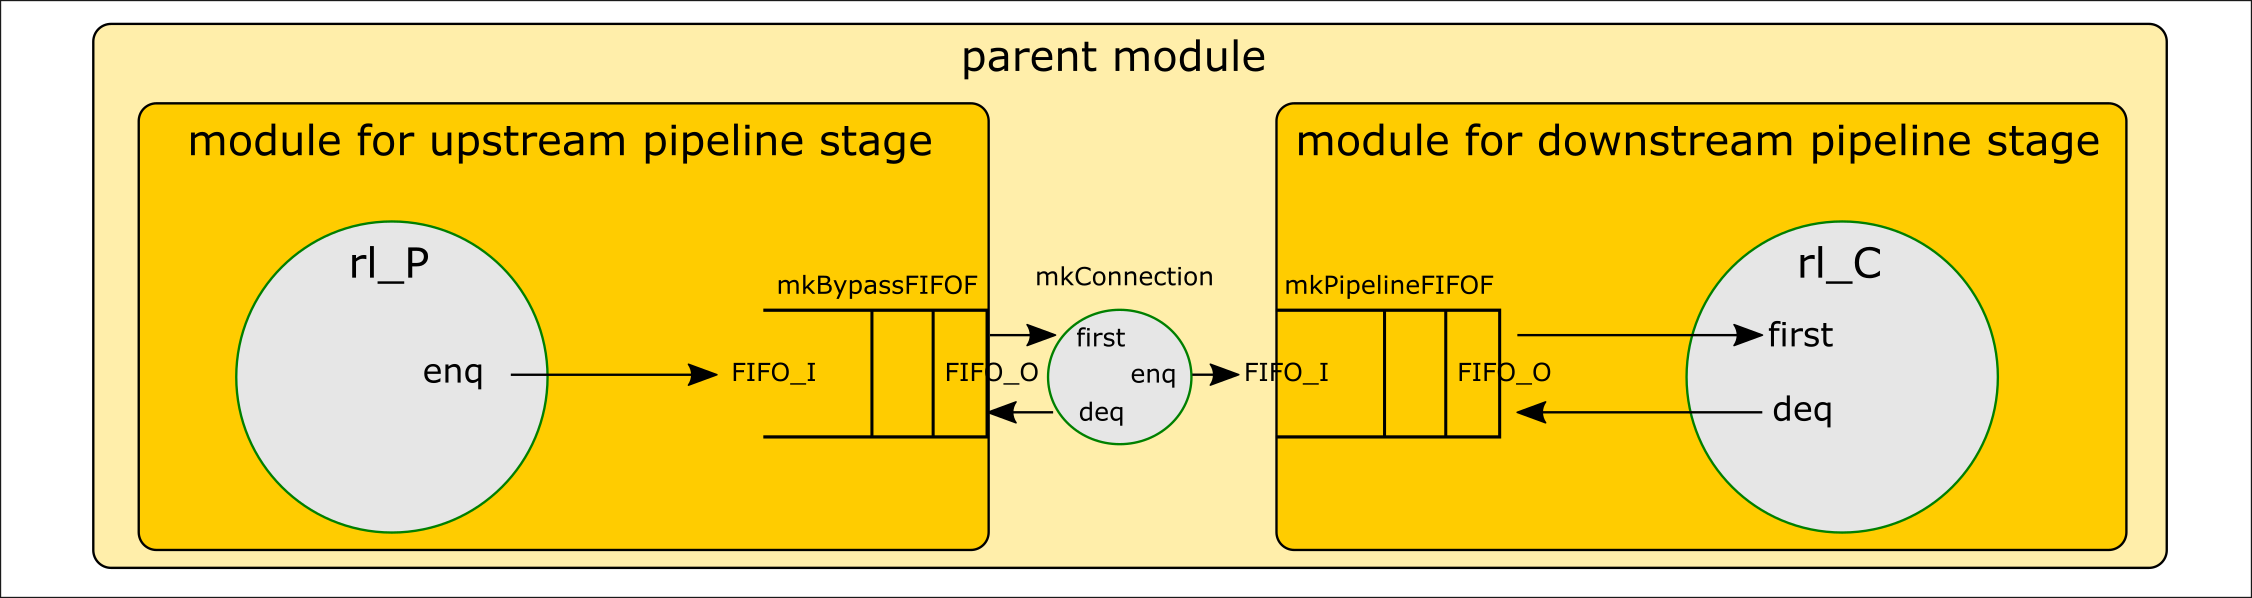
\includegraphics[width=\textwidth]{Fig_Composed_FIFO_modularity}
\end{minipage}

\PAUSE{\vspace{2ex}}

\begin{itemize}

 \item Data can traverse from producer to consumer in 1 tick, as
       desired, despite there being two FIFOs, because of the
       semantics of {\tt mkBypassFIFOF} and {\tt mkPipelineFIFOF}
       (Chapter 17).

 \item The structure allows the producer and consumer to be compiled
       independently by \emph{bsc}, with no ``rule-scheduling''
       constraints leaking across stage boundaries.

 \item There are no combinational paths crossing the stage boundary
       (through the two FIFOs).

 \item The structure allows us to reason about correctness of each
       stage completely independently of other stages.

\end{itemize}

\end{frame}

% ================================================================

\begin{frame}[fragile]
\frametitle{Fife module interface definitions}

\footnotesize

\begin{minipage}{0.75\textwidth}\scriptsize
\begin{Verbatim}[frame=single, label=From src\_Fife/CPU.bsv]
   method Action init (Initial_Params initial_params);
      rg_flog <= initial_params.flog;

      stage_F.init (initial_params);
      stage_D.init (initial_params);
      stage_RR_RW.init (initial_params);
      stage_EX_Control.init (initial_params);
      stage_EX_Int.init (initial_params);
      stage_Retire.init (initial_params);
   endmethod

   // IMem
   interface fo_IMem_req = stage_F.fo_Fetch_to_IMem;
   interface fi_IMem_rsp = stage_D.fi_IMem_to_Decode;

   // DMem, speculative
   interface fo_DMem_S_req    = stage_RR_RW.fo_DMem_S_req;
   interface fi_DMem_S_rsp    = stage_Retire.fi_DMem_S_rsp;
   interface fo_DMem_S_commit = stage_Retire.fo_DMem_S_commit;

   // DMem, non-speculative
   interface fo_DMem_req = stage_Retire.fo_DMem_req;
   interface fi_DMem_rsp = stage_Retire.fi_DMem_rsp;

   // Set TIME
   method Action set_TIME (Bit #(64) t) = stage_Retire.set_TIME (t);
\end{Verbatim}
\end{minipage}
\hm
\begin{minipage}{0.22\textwidth}
The {\tt init} method initializes this module and also each stage sub-module.

\vspace{2ex}

The {\tt set\_TIME} method is for updating the {\tt time} CSR.
\end{minipage}

\end{frame}

% ****************************************************************

\section{Fetch stage}

\begin{frame}[fragile]

\begin{center}
  {\LARGE Fife CPU Fetch stage}

  \vspace{10ex}

  Please simultaneously view file: \hm \verb|Code/src_Fife/S1_Fetch.bsv|
\end{center}

\end{frame}

% ================================================================

\begin{frame}[fragile]
\frametitle{Fetch stage: interface}

\footnotesize

\begin{minipage}{0.725\textwidth}
\SHOWCODE{../Code_Extracts/Fife_Fetch_IFC.tex}
\end{minipage}
\begin{minipage}{0.25\textwidth}
Interface

\vspace{5ex}

The \verb|FIFO_I| from Retire carries redirection information (update
PC on misprediction/exception/interrupt).

\end{minipage}

\end{frame}

% ================================================================

\begin{frame}[fragile]
\frametitle{Fetch stage: implementation module}

\footnotesize

For module {\tt mkFetch} let us examine file: \verb|Code/src_Fife/S1_Fetch.bsv|

\vspace{4ex}

\begin{itemize}

 \item Rule \verb|rl_Fetch_req| is the forward-flow ``fetching rule'',
       repeatedly invoking \verb|fn_Fetch| to produce IMem requests
       and information for Decode.

       The expression ``\verb|rg_pc+4|'' is, more generally,
       ``\verb|predict(rg_pc)|''.

       In future we can substitute new, improved, predictor functions
       (see book ``Section 18.3.6.4 Better next-PC prediction'').

 \item Rule \verb|rl_Fetch_from_Retire| is the backward-flow.  It
       receives \verb|Fetch_from_Retire| messages from Retire whenever
       Retire needs to change the control flow to something other than
       the predicted PC (due to BRANCH, JAL, JALR, or traps).  This
       rule updates \verb|rg_pc| to the newly specified PC, and also
       updates \verb|rg_epoch|.

 \vspace{4ex}

 \item The expression \verb|(! f_Fetch_from_Retire.notEmpty)|
       in \verb|rl_Fetch_req|'s condition gives it lower priority
       compared to \verb|rl_Fetch_from_Retire| when both are enabled.
       The sooner we perform redirection, the fewer wrong-path
       instructions will be fetched.

\end{itemize}

\vspace{4ex}

{\tt rg\_oiaat} is used for ``one instruction at a time'' mode (for
debugging), and can be ignored for now.

\end{frame}

% ****************************************************************

\section{Decode stage}

\begin{frame}[fragile]

\begin{center}
  {\LARGE Fife CPU Decode stage}

  \vspace{10ex}

  Please simultaneously view file: \hm \verb|Code/src_Fife/S2_Decode.bsv|
\end{center}

\end{frame}

% ================================================================

\begin{frame}[fragile]
\frametitle{Decode stage: interface}

\footnotesize

\begin{minipage}{0.725\textwidth}
\SHOWCODE{../Code_Extracts/Fife_Decode_IFC.tex}
\end{minipage}
\hmm
Interface

\end{frame}

% ================================================================

\begin{frame}[fragile]
\frametitle{Decode stage: implementation module}

\footnotesize

For module {\tt mkDecode} code, let us examine file: \verb|Code/src_Fife/S2_Decode.bsv|

\begin{itemize}

\vspace{4ex}

 \item FIFO \verb|f_Fetch_to_Decode| is a {\tt mkSizedFIFO(4)}
       instance, aiming to balance the Fetch-to-Decode direct path
       length with the Fetch-to-IMem-to-Decode path length (equalize
       the number of items that can be ``in flight'' on each path).

 \vspace{5ex}

 \item Rule \verb|rl_Decode| is the forward-flow;
       it repeatedly invokes \verb|fn_Decode| to produce
       information for the next stage.

\end{itemize}

\end{frame}

% ****************************************************************

\section{Register-Read and Dispatch stage (and Register-Write)}

\begin{frame}[fragile]

\begin{center}
  {\LARGE Fife CPU Register-Read and Dispatch stage \\
          (and Register-Write)}

  \vspace{10ex}

  Please simultaneously view file: \hm \verb|Code/src_Fife/S3_RR_RW.bsv|
\end{center}

\end{frame}

% ================================================================

\begin{frame}[fragile]
\frametitle{Register-Read and Dispatch stage (and Register-Write): Interface}

\footnotesize

\begin{minipage}{0.725\textwidth}
\SHOWCODE{../Code_Extracts/Fife_RR_RW_IFC.tex}
\end{minipage}
\hfill
\begin{minipage}{0.25\textwidth}
Interface

\vspace{2ex}

The four \verb|FIFO_O| interfaces feed the four execution paths.

\vspace{2ex}

The \verb|FIFO_I| from Retire carries information for register-write
and release of scoreboard reservations.
\end{minipage}

\end{frame}

% ================================================================

\begin{frame}[fragile]
\frametitle{Reg-Read and Dispatch (and Reg-Write): GPRs}

\footnotesize

For module {\tt mkRR\_RW} code, let us examine file: {\tt Code/src\_Fife/S3\_RR\_RW.bsv}

\begin{center}
 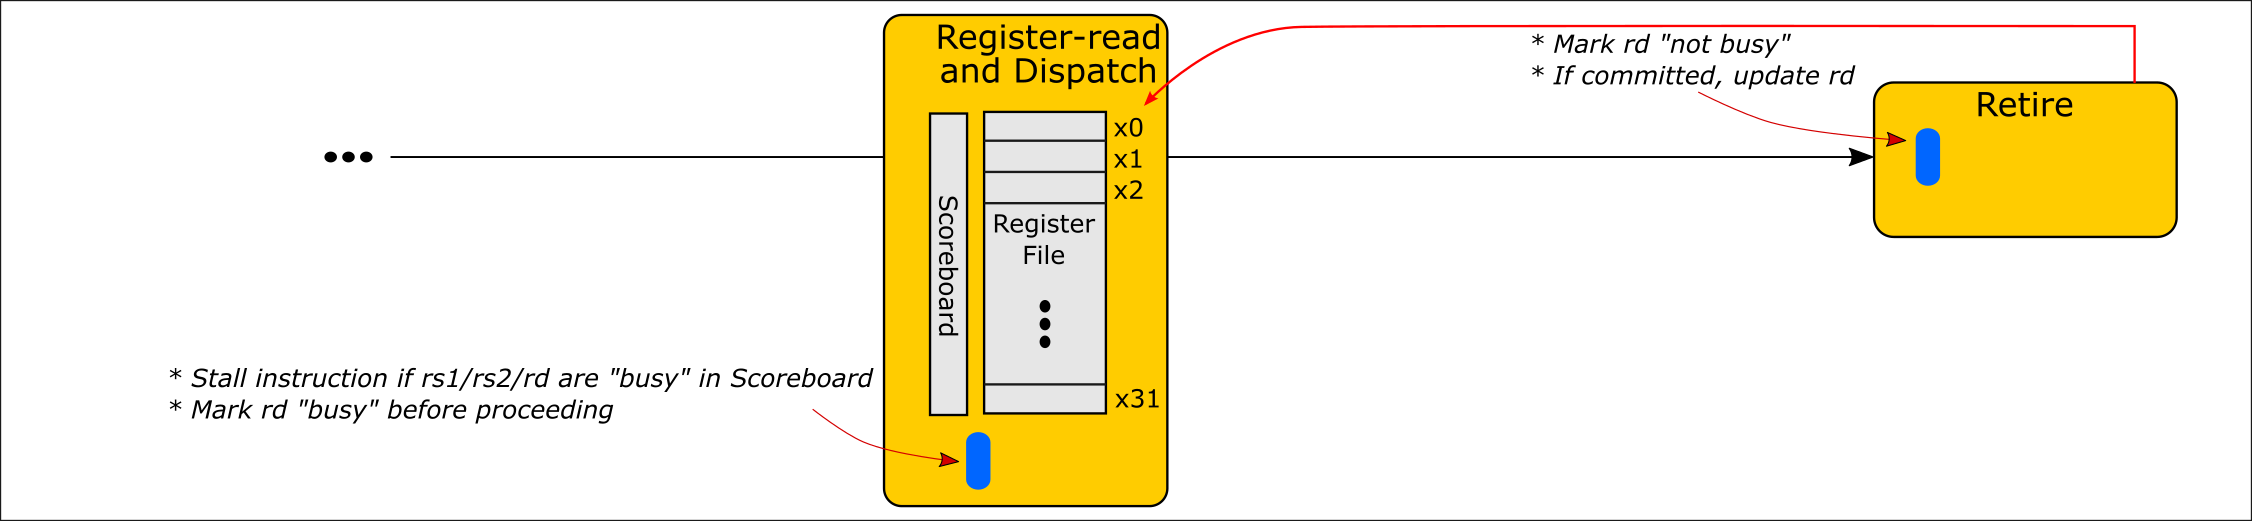
\includegraphics[width=0.8\textwidth]{Fig_RISCV_Scoreboard}
\end{center}

\vspace{2ex}

The GPRs (general-purpose registers) are instantiated in this module
because we will be reading Rs1 and Rs2 here for each instruction:

\vspace{2ex}

\begin{Verbatim}[frame=single, label=From src\_Fife/CPU.bsv]
   GPRs_IFC #(XLEN)  gprs <- mkGPRs_synth;
\end{Verbatim}

\vspace{2ex}

{\tt mkGPRS\_synth} is just a version of {\tt mkGPRs} instantiated
with a specific {\tt XLEN} width, and with the {\tt (* synthesize *)}
attribute so that it becomes a Verilog module.

\end{frame}

% ================================================================

\begin{frame}[fragile]
\frametitle{Reg-Read and Dispatch (and Reg-Write): Scoreboard}

\footnotesize

\begin{center}
 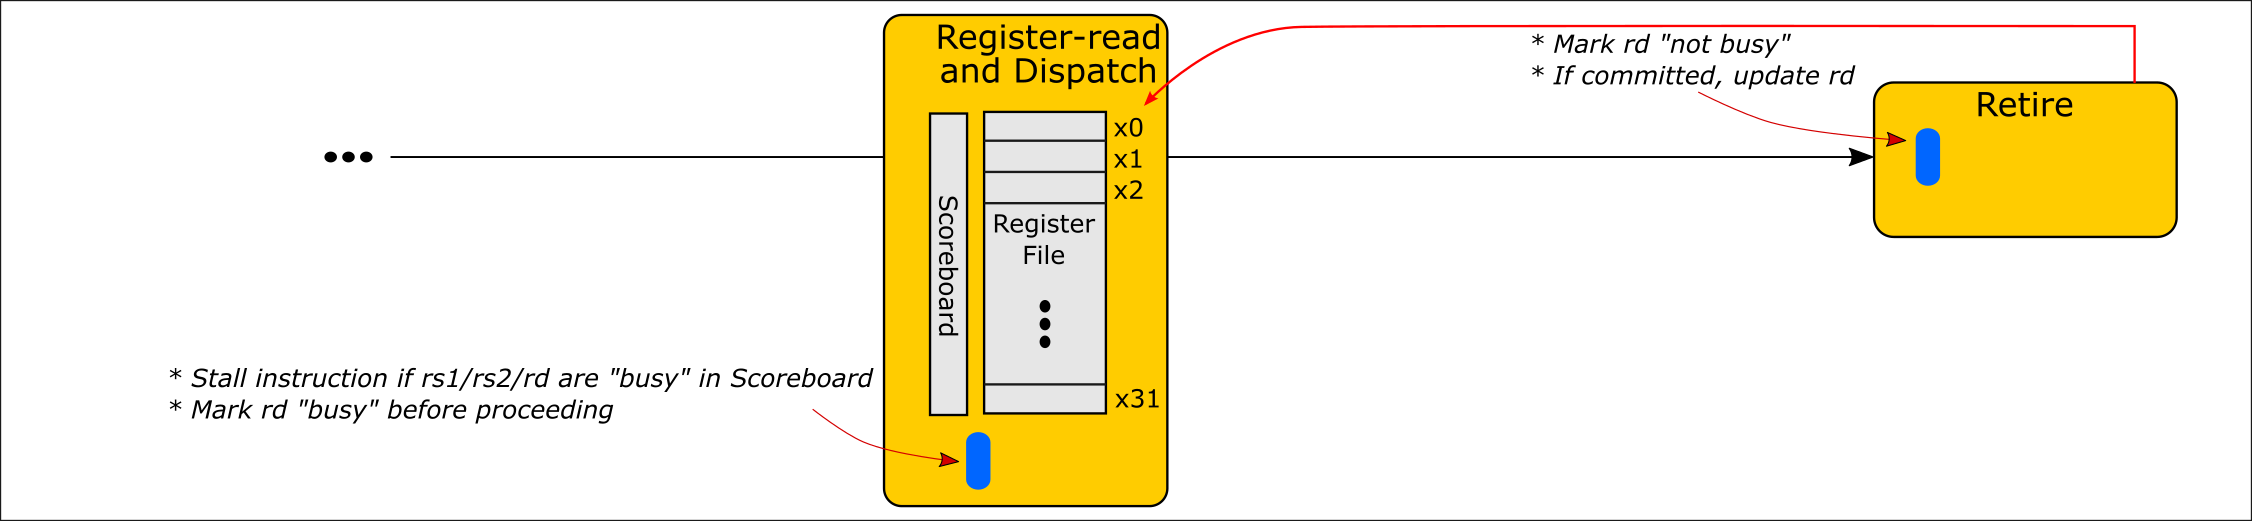
\includegraphics[width=0.8\textwidth]{Fig_RISCV_Scoreboard}
\end{center}

\vspace{2ex}

The Scoreboard accompanies the GPRs.  It contains one bit per GPR,
indicating whether it is busy (1) or not-busy (0).

\vspace{2ex}

\begin{Verbatim}[frame=single, label=From src\_Fife/CPU.bsv]
typedef  Vector #(32, Bit #(1))  Scoreboard;

Reg #(Scoreboard) rg_scoreboard <- mkReg (replicate (0));
\end{Verbatim}

\vspace{2ex}

(Type {\tt Vector\#($n$,$t$)} represents a vector of $n$ elements, each of type $t$.)

\end{frame}

% ================================================================

\begin{frame}[fragile]
\frametitle{Reg-Read and Dispatch (forward flow)}

\footnotesize

Let us examine {\tt rl\_RR\_Dispatch} in file: {\tt Code/src\_Fife/S3\_RR\_RW.bsv}

\vspace{2ex}

\begin{itemize}

  \item It stalls (waits) if the instruction has Rs1, Rs2 or Rd, and
        these are busy according to the scoreboard.

  \item Othersize

    \begin{itemize}\footnotesize
      \item It reads Rs1 and Rs2 registers for the current instruction.

      \vspace{1ex}

      \item It sets the scoreboard for the current instruction's Rd to
            1, marking it ``busy'' (if the instruction has an Rd);

      \vspace{1ex}

      \item It uses information from Decode to dispatch to the four
            Execute pipes.  We always (for every instruction) send an
            execution tag and additional information on the direct
            pipe.  Depending on the instruction, it may also send
            information into one of the other Execute pipes: (Execute
            Control, Execute Integer, and DMem)
    \end{itemize}

\end{itemize}

\end{frame}

% ================================================================

\begin{frame}[fragile]
\frametitle{Reg-Write (backward flow)}

\footnotesize

Let us examine {\tt rl\_RW\_from\_Retire} in file: {\tt Code/src\_Fife/S3\_RR\_RW.bsv}

\vspace{2ex}

\begin{itemize}

 \item We pop the message \verb|x| from the \verb|f_RW_from_Retire| FIFO.

 \item We perform its specified scoreboard-release for register Rd.
       If the Rd value is to be committed, we write it into GPR [Rd].

\end{itemize}

\vspace{5ex}

The two rules \verb|rl_RR_Dispatch| and \verb|rl_RW_from_Retire| run concurrently.

\vspace{2ex}

If \verb|rl_RR_Dispatch| was stalled on an instruction whose Rs1 or
Rs2 was busy, executing \verb|rl_RW_from_Retire| may ``un-stall'' it,
if its Rd-write is to the pending register.

\vspace{1ex}



The explicit condition on \verb|rl_RR_Dispatch|:
\begin{center}
\verb|(! f_RW_from_Retire.notEmpty)|
\end{center}
prioritizes the forward rule lower than the backward
rule \verb|rl_RW_from_Retire|, so that this ``un-stalling'' (if it
happens) can happen as soon as possible.

\end{frame}

% ****************************************************************

\section{Execute Control stage}

\begin{frame}[fragile]

\begin{center}
  {\LARGE Fife CPU Execute Control stage}

  \vspace{10ex}

  Please simultaneously view file: \hm \verb|Code/src_Fife/S4_EX_Control.bsv|
\end{center}

\vspace{5ex}

This is a very simple, forward-flow-only, one-in, one-out module; it
 just applies \verb|fn_EX_Control()| (which we have already seen in
 Drum) to each item as it transits.

\end{frame}

% ****************************************************************

\section{Execute Int stage}

\begin{frame}[fragile]

\begin{center}
  {\LARGE Fife CPU Execute Int stage}

  \vspace{10ex}

  Please simultaneously view file: \hm \verb|Code/src_Fife/S4_EX_Int.bsv|
\end{center}

\vspace{5ex}

This is a very simple, forward-flow-only, one-in, one-out module; it
 just applies \verb|fn_EX_Int()| (which we have already seen in Drum)
 to each item as it transits.

\end{frame}

% ****************************************************************

\section{Retire stage}

\begin{frame}[fragile]

\begin{center}
  {\LARGE Fife CPU Retire stage}

  \vspace{10ex}

  Please simultaneously view file: \hm \verb|Code/src_Fife/S5_Retire.bsv|
\end{center}

\end{frame}

% ================================================================

\begin{frame}[fragile]
\frametitle{Retire stage module interface}

\footnotesize

\begin{minipage}{0.725\textwidth}
\SHOWCODESCRIPT{../Code_Extracts/Fife_Retire_IFC.tex}
\end{minipage}

\end{frame}

% ================================================================

\begin{frame}[fragile]
\frametitle{Retire stage flows}

\footnotesize

\begin{center}
 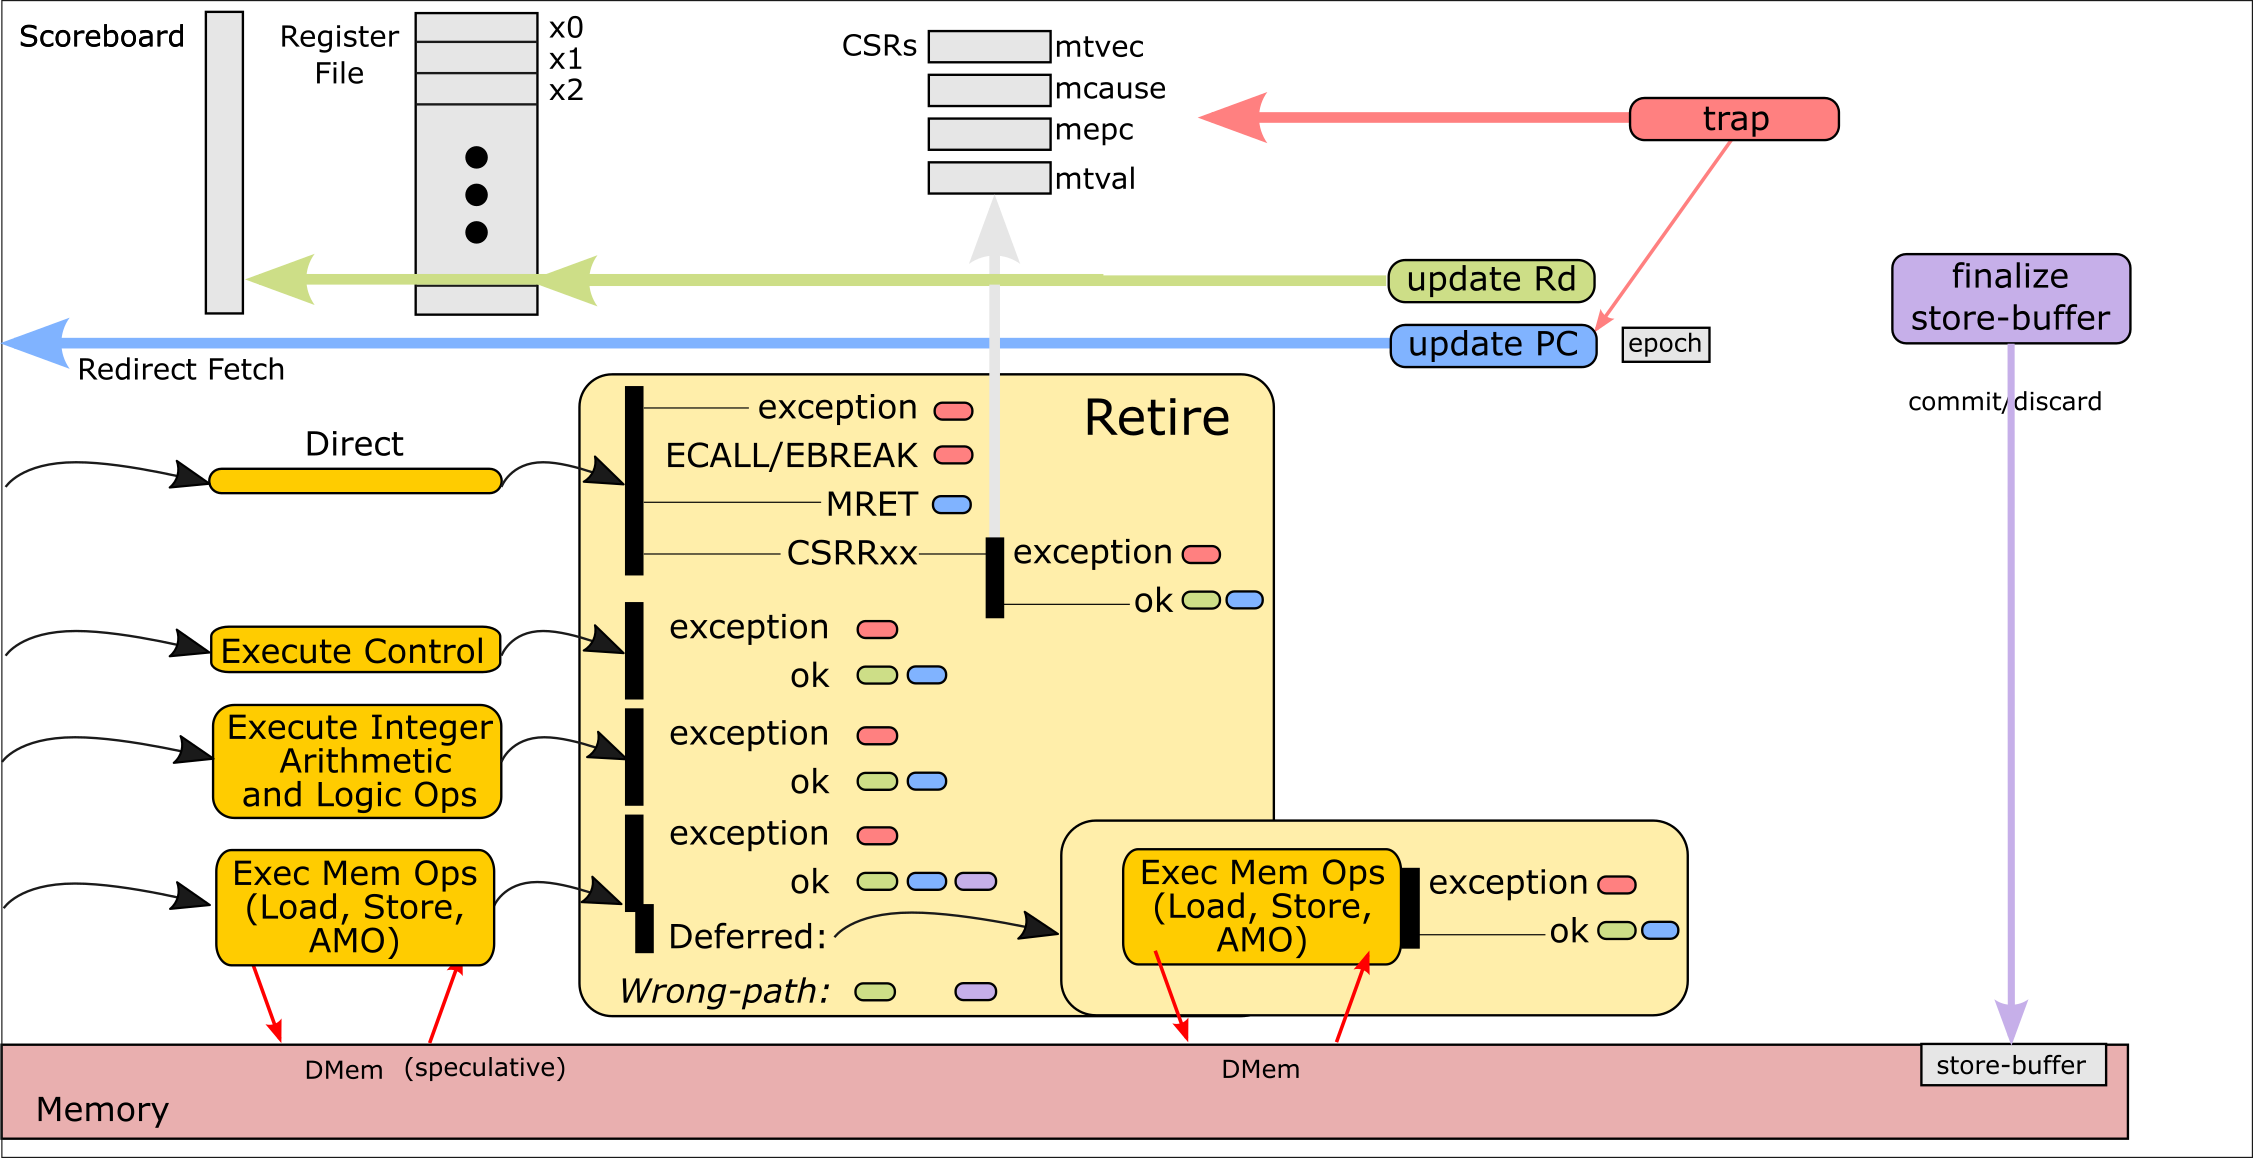
\includegraphics[width=0.9\textwidth]{Fig_Retire_Layers_1_2}
\end{center}

\end{frame}

% ================================================================

\begin{frame}[fragile]
\frametitle{Retire stage module ``mode''}

\footnotesize

Normally, the Retire stage retires an instruction on every clock (\verb|MODE_PIPE|).

\emph{Except}

\begin{itemize}

 \item For DMem ``Deferred'' instructions (for MMIO), \\
       we send the DMem request, and \\
       transition to \verb|MODE_DMEM_RSP|.

       In \verb|MODE_DMEM_RSP| we collect the DMem response, \\
       retire the instruction, \\
       and return to \verb|MODE_PIPE|.

 \item For exceptions, we transition to \verb|MODE_EXCEPTION|.

       In \verb|MODE_EXCEPTION| we perform the trap actions, \\
       and return to \verb|MODE_PIPE|.
\end{itemize}

\vspace{5ex}

\begin{minipage}{0.725\textwidth}
\SHOWCODESCRIPT{../Code_Extracts/Fife_Retire_Module_Mode}
\end{minipage}

\end{frame}

% ================================================================

\begin{frame}[fragile]
\frametitle{Retire stage module state: highlights}

\footnotesize

\begin{minipage}{0.725\textwidth}
\begin{Verbatim}[frame=single, label=From Code/src\_Fife/S5\_Retire.bsv]
module mkRetire (Retire_IFC);
   ...
   // Control-and-Status Registers (CSRs)
   CSRs_IFC csrs <- mkCSRs;

   // For managing speculation, redirection, traps, etc.
   Reg #(Epoch) rg_epoch  <- mkReg (0);
   ...
   ... FIFOs for incoming and outgoing flows ...
   ...
   Reg #(Module_Mode) rg_mode <- mkReg (MODE_PIPE);

   ...

endmodule
\end{Verbatim}
\end{minipage}

\end{frame}

% ================================================================

\begin{frame}[fragile]
\frametitle{Retire stage module: help-functions and useful predicates}

\footnotesize

\begin{minipage}{0.725\textwidth}
\begin{Verbatim}[frame=single, label=From Code/src\_Fife/S5\_Retire.bsv]
module mkRetire (Retire_IFC);
   ...
   function Action fa_redirect_Fetch (...);
   ...
   function Action fa_update_rd (...);
   ...
   function Action fa_retire_store_buf (...);
   ...
   RR_to_Retire x_rr_to_retire = f_RR_to_Retire.first;

   Bool wrong_path = (x_rr_to_retire.epoch != rg_epoch);
   Bool is_Direct  = (x_rr_to_retire.exec_tag == EXEC_TAG_DIRECT);
   Bool is_Control = (x_rr_to_retire.exec_tag == EXEC_TAG_CONTROL);
   Bool is_Int     = (x_rr_to_retire.exec_tag == EXEC_TAG_INT);
   Bool is_DMem    = (x_rr_to_retire.exec_tag == EXEC_TAG_DMEM);
   ...
endmodule
\end{Verbatim}
\end{minipage}

\end{frame}

% ================================================================

\begin{frame}[fragile]
\frametitle{Retire stage module: rule for wrong-path instructions (mispredicted)}

\footnotesize

\begin{minipage}{0.725\textwidth}
\SHOWCODESCRIPT{../Code_Extracts/Fife_rl_wrong_path}
\end{minipage}

\end{frame}

% ================================================================

\begin{frame}[fragile]
\frametitle{Retire stage module: rules for Direct path instructions (1/2)}

\footnotesize

\begin{minipage}{0.725\textwidth}\scriptsize
\begin{Verbatim}[frame=single, label=From Code/src\_Fife/S5\_Retire.bsv]
   rule rl_Retire_CSRRxx ((rg_mode == MODE_PIPE)
			  && (! wrong_path)
			  && is_Direct
			  && (! x_rr_to_retire.exception)
			  && is_legal_CSRRxx (x_rr_to_retire.instr));
      ...
      match { .exc, .rd_val } <- csrs.mav_csrrxx (...);
      ...
      if (! exc)
	 ...
      else begin
	 ...
	 rg_mode  <= MODE_EXCEPTION;
      end
   endrule
\end{Verbatim}
\end{minipage}

\vspace{2ex}

\begin{minipage}{0.725\textwidth}\scriptsize
\begin{Verbatim}[frame=single, label=From Code/src\_Fife/S5\_Retire.bsv]
   rule rl_Retire_MRET ((rg_mode == MODE_PIPE)
			&& (! wrong_path)
			&& is_Direct
			&& (! x_rr_to_retire.exception)
			&& is_legal_MRET (x_rr_to_retire.instr));
      ...
   endrule
\end{Verbatim}
\end{minipage}

\end{frame}

% ================================================================

\begin{frame}[fragile]
\frametitle{Retire stage module: rules for Direct path instructions (2/2)}

\footnotesize

\begin{minipage}{0.725\textwidth}\scriptsize
\begin{Verbatim}[frame=single, label=From Code/src\_Fife/S5\_Retire.bsv]
   rule rl_Retire_ECALL_EBREAK ((rg_mode == MODE_PIPE)
				&& (! wrong_path)
				&& is_Direct
				&& (! x_rr_to_retire.exception)
				&& (is_legal_ECALL (x_rr_to_retire.instr)
				    || is_legal_EBREAK (x_rr_to_retire.instr)));
      ...
      rg_mode <= MODE_EXCEPTION;
      ...
   endrule

   rule rl_Retire_Direct_exception ((rg_mode == MODE_PIPE)
				    && (! wrong_path)
				    && is_Direct
				    && x_rr_to_retire.exception);
      ...
      rg_mode <= MODE_EXCEPTION;
      ...
   endrule
\end{Verbatim}
\end{minipage}

\end{frame}

% ================================================================

\begin{frame}[fragile]
\frametitle{Retire stage module: rules for Execute Control and Int paths instructions}

\footnotesize

\begin{minipage}{0.725\textwidth}\scriptsize
\begin{Verbatim}[frame=single, label=From Code/src\_Fife/S5\_Retire.bsv]
   rule rl_Retire_EX_Control ((rg_mode == MODE_PIPE)
			      && (! wrong_path)
			      && is_Control);
      ...
      if (! x2.exception)
	 ...
      else begin
	 ...
	 rg_mode <= MODE_EXCEPTION;
      end
   endrule
\end{Verbatim}
\end{minipage}

\vspace{2ex}

\begin{minipage}{0.725\textwidth}\scriptsize
\begin{Verbatim}[frame=single, label=From Code/src\_Fife/S5\_Retire.bsv]
   rule rl_Retire_EX_Int ((rg_mode == MODE_PIPE)
			  && (! wrong_path)
			  && is_Int);
      ...
      if (! x2.exception)
	 ...
      else begin
	 ...
	 rg_mode <= MODE_EXCEPTION;
      end
   endrule
\end{Verbatim}
\end{minipage}

\end{frame}

% ================================================================

\begin{frame}[fragile]
\frametitle{Retire stage module: rules for Execute DMem path instructions (1/2)}

\footnotesize

\begin{minipage}{0.725\textwidth}\scriptsize
\begin{Verbatim}[frame=single, label=From Code/src\_Fife/S5\_Retire.bsv]
   rule rl_Retire_EX_DMem ((rg_mode == MODE_PIPE)
			   && (! wrong_path)
			   && is_DMem
			   && (f_DMem_S_rsp.first.rsp_type != MEM_REQ_DEFERRED));
      ...
      if (! exception)
	 ...
      else begin
	 ...
	 rg_mode <= MODE_EXCEPTION;
      end
   endrule
\end{Verbatim}
\end{minipage}

\vspace{2ex}

\begin{minipage}{0.725\textwidth}\scriptsize
\begin{Verbatim}[frame=single, label=From Code/src\_Fife/S5\_Retire.bsv]
   rule rl_Retire_DMem_deferred ((rg_mode == MODE_PIPE)
				 && (! wrong_path)
				 && is_DMem
				 && (f_DMem_S_rsp.first.rsp_type
				     == MEM_REQ_DEFERRED));
      ...
      f_DMem_req.enq (mem_req);
      rg_mode <= MODE_DMEM_RSP;    // go to await response
   endrule
\end{Verbatim}
\end{minipage}

\end{frame}

% ================================================================

\begin{frame}[fragile]
\frametitle{Retire stage module: rules for Execute DMem path instructions (2/2)}

\footnotesize

\begin{minipage}{0.725\textwidth}
\begin{Verbatim}[frame=single, label=From Code/src\_Fife/S5\_Retire.bsv]
   rule rl_Retire_DMem_rsp (rg_mode == MODE_DMEM_RSP);
      ...
      if (exception) begin
	 ...
	 rg_mode <= MODE_EXCEPTION;
      end
      else begin
	 ...
	 rg_mode <= MODE_PIPE;
      end
   endrule
\end{Verbatim}
\end{minipage}

\end{frame}

% ================================================================

\begin{frame}[fragile]
\frametitle{Retire stage module: rule for exception-handling}

\footnotesize

\SHOWCODE{../Code_Extracts/Fife_S5_exc}

\end{frame}

% ****************************************************************

\section{Final Comments}

\begin{frame}[fragile]
\frametitle{Fife CPU: final comments}

\footnotesize

\begin{itemize}

 \item There is very little in this chapter that is RISC-V specific;
       these pipeline structures are needed for a pipelined CPU for
       any ISA. All RISC-V-specific issues are the same as in Drum.

 \PAUSE{\vspace{5ex}}

 \item Much scope for performance optimization. {\Eg}

    \begin{itemize}\footnotesize

      \item Faster delivery of redirection to Fetch (less wrong-path wastage)

      \item Faster delivery of Rd value to Register-Read (less stalling)

      \item In Retire, handle exceptions earlier except perhaps in CSRRxx case.
    \end{itemize}

    These are discussed further in Chapter 17.

\end{itemize}

\end{frame}

% ****************************************************************

% -*- mode: fundamental -*-

% Slides accompanying "Learn RISC-V CPU Implementation and BSV" book
% Copyright (c) 2024 Rishiyur S. Nikhil, All Rights Reserved

% This is a postamble shared by all the slide decks

% ================================================================

\begin{frame}

\begin{center}
  {\LARGE End}
\end{center}

\end{frame}

% ================================================================


% ****************************************************************

\end{document}
% ****************************************************************
